\chapter{Implementácia}

\section{Metóda RISEI}

Metódu RISEI sme sa rozhodli implementovať v jazyku Python, keďže plánujeme používať knižnice pre strojové učenie akými sú \textit{tensorflow} či \textit{scikit-learn}.

\subsection{Generovanie masiek}

Na základe BPMN diagramu (Obr. \ref{fig:risei_diagram}) sme implementovali proces generovania masiek. Generovanie masiek môže prebiehať paralelne vo viacerích procesoch použitím knižnice Python \textit{multiprocessing}. V tejto sekcii popíšeme jednotlivé kroky.

\paragraph{Vytvorenie náhodnej binárnej masky}

Náhodné binárne masky generujeme pomocou knižnice \textit{numpy}. Pomocou nasledovného kódu vygenerujeme $N$ náhodných masiek 3D binárnych matíce. Obr. \label{fig:risei_inpainting_example} zobrazuje takúto binárnu maticu, ale v 2D. \textit{size} (veľkosť) a \textit{probability} (pravdepodobnosť) sú hyper-parametrami RISEI metódy. \textit{size} hovorí o veľkosti generovanej masky, čím je toto číslo väčšie tým bude výsledná maska viac fragmentovaná na malé plochy. \textit{probability} hovorí o tom, s akou pravdepodobnosťou daná plocha neprekrytá maskou. RISE používa predvolenú hodnotu \textit{size = 8}.

\begin{lstlisting}
    binary_masks = np.random.rand(N, size, size, size) < probability
\end{lstlisting}

\begin{figure}[h!]
    \centering
    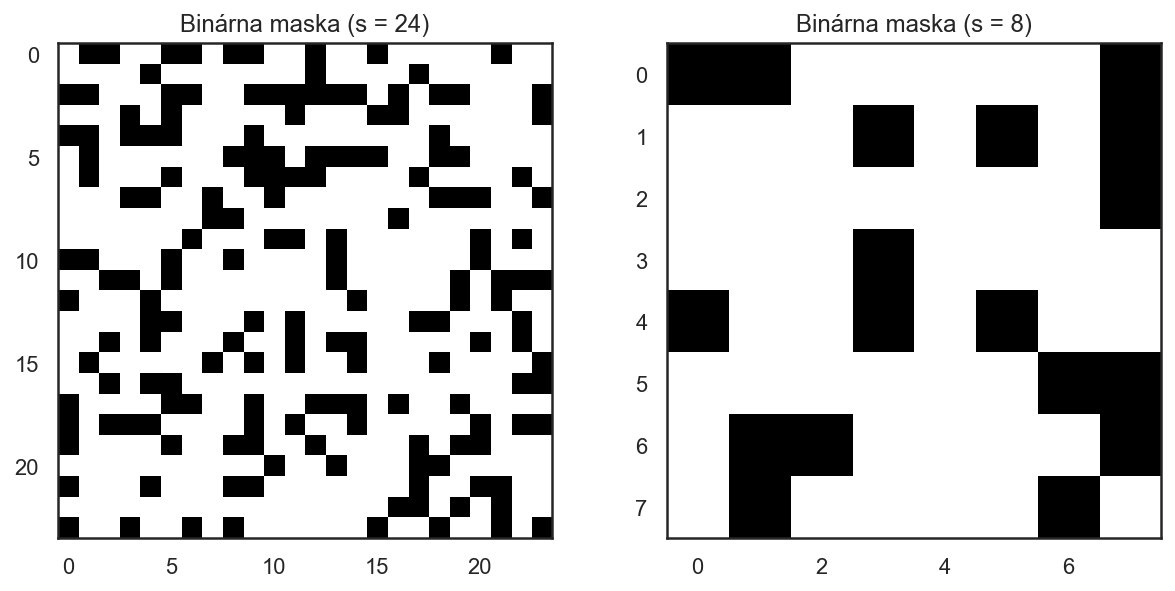
\includegraphics[width=13cm]{assets/images/binary_mask.png}
    \caption{Porovnanie dvoch binárnych masiek s rôznou veľkosťou (\textit{size}), čím väčšia veľkosť, tým je obrázok viac fragmentovaný.}
    \label{fig:binary_mask}
\end{figure}

\paragraph{Náhodné nastavenie pozície vyrezania, zväčšenie binárnej masky a orezenie na veľkosť obrázka}

Binárnu masku zväčšíme na veľkosť vstupného snímku plus menší offset (o veľkosti size). Následne zo zväčšenej masky na náhodnej pozícii vyrežeme masku o veľkosti vstupného snímku (Obr. \ref{fig:binary_mask_resized}). Táto maska určuje, ktoré miesta na snímku bude treba dokresliť - biele miesta, čiže jednotky. Tento krok v pôvodnej implementácii RISE nie je.

\begin{figure}[h!]
    \centering
    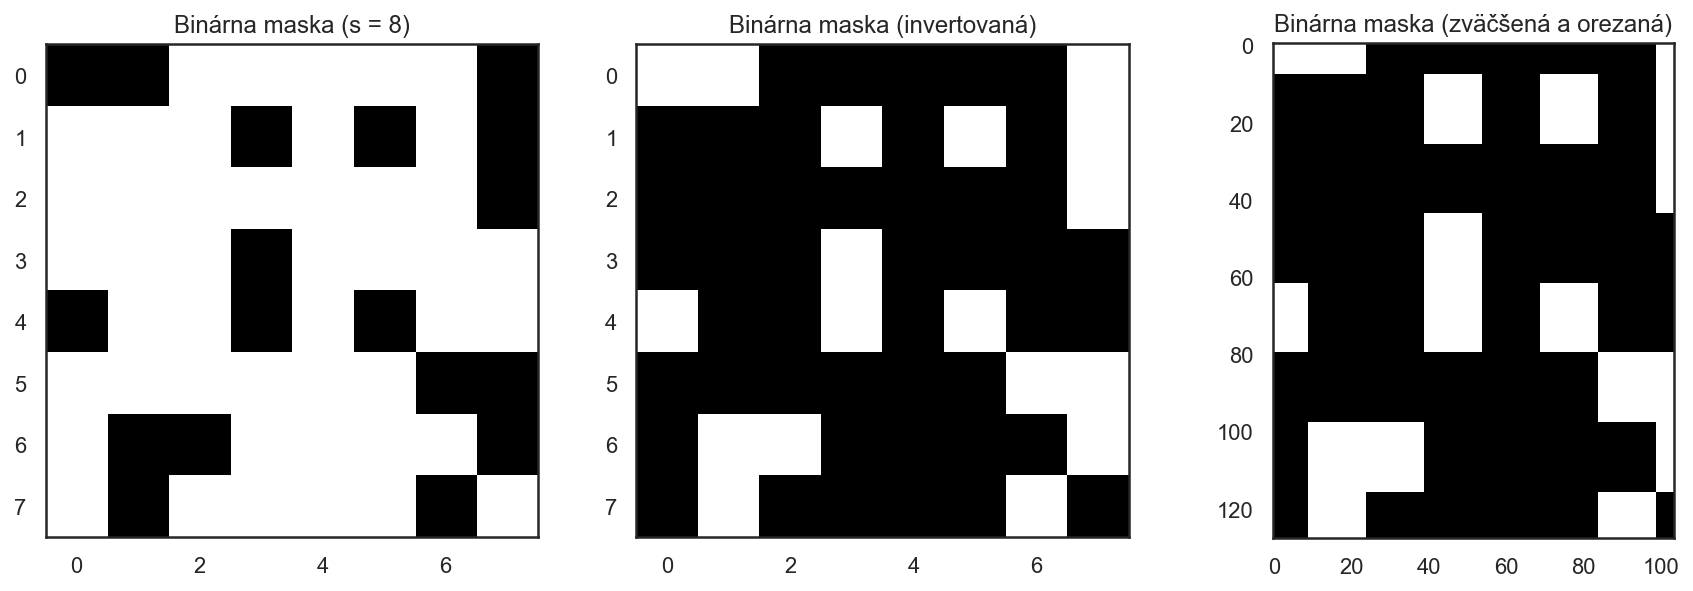
\includegraphics[width=13cm]{assets/images/binary_mask_resized.png}
    \caption{Vygenerovaná maska je zväčšená a orezaná na veľkosť vstupného snímku (ten je o veľkosti $[104, 128, 104]$ pričim na obrázkoch je vizualizovaná druhá a tretia dimenzia). Úplne vľavo je binárna maska o veľkosti $8$. V strede je invertovaná binárna maska (kvôli ďaľšiemu pracovanou s ňou) a vpravo je orezaná binárna maska o veľkosti vstupného snímku.}
    \label{fig:binary_mask_resized}
\end{figure}

\paragraph{Zväčšenie pomocou bilineárnej interpolácie a orezanie masky na veľkosť obrázka}

Tak ako v poôvodnej implementácii RISE, vytvoríme ''čiernu'' masku na zakrytie častí obrázku. Pôvodnú binárnu masku pomocou bilineárnej interpolácie (funkcia \textit{resize} z knižnice \textit{scikit-learn}) zväčšíme na veľkost vstupného snímku plus menší offset, následne vyrežeme na náhodnej pozicii masku o veľkosti vstupného snímku (táto náhodná pozícia je rovnaká ako pri orezávani binárnej masky bez interpolácie, preto je v BPMN diagrame v samostatnom kroku).

\begin{figure}[h!]
    \centering
    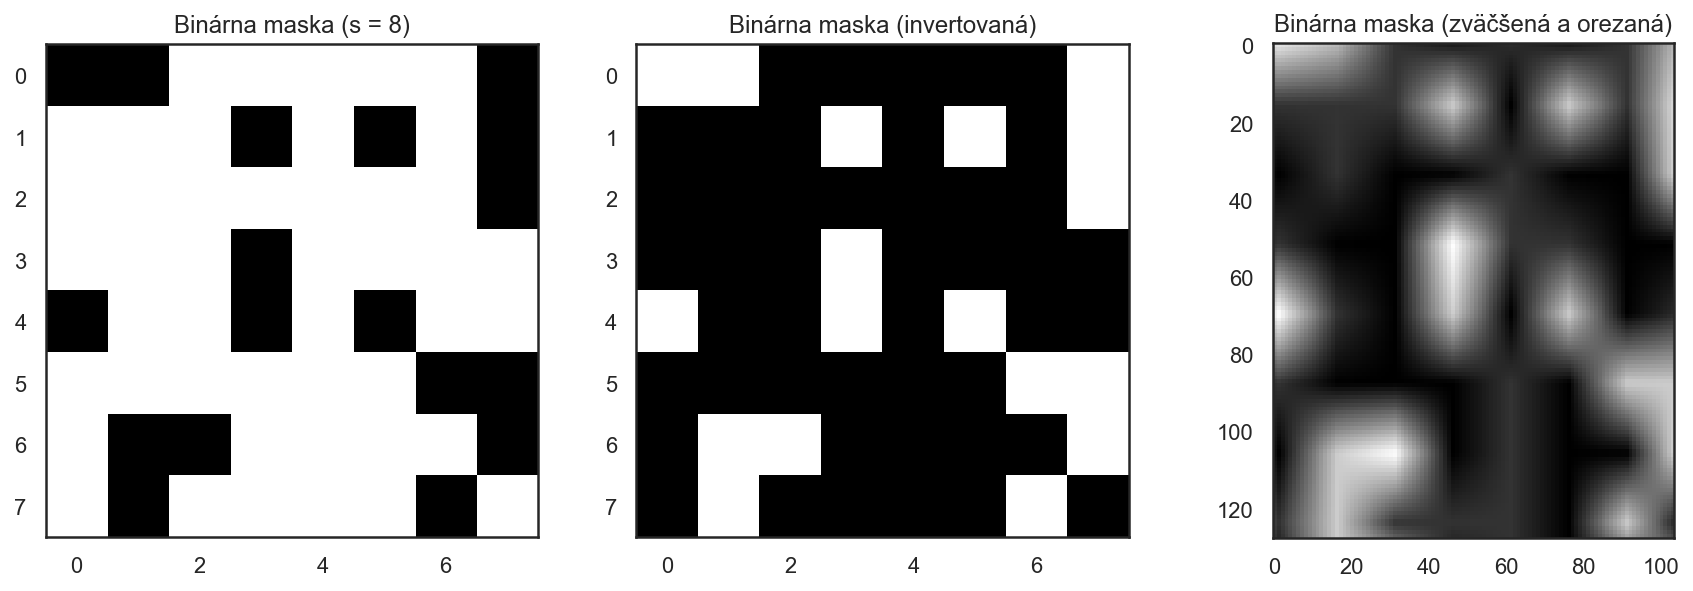
\includegraphics[width=13cm]{assets/images/interpolated_mask.png}
    \caption{Vygenerovaná maska je zväčšená pomocou bilineárnej interpolácie a orezaná na veľkosť vstupného snímku (ten je o veľkosti $[104, 128, 104]$ pričim na obrázkoch je vizualizovaná druhá a tretia dimenzia). Úplne vľavo je binárna maska o veľkosti $8$. V strede je invertovaná binárna maska (kvôli ďaľšiemu pracovanou s ňou) a vpravo je orezaná interpolovaná ''čierna'' maska o veľkosti vstupného snímku.}
    \label{fig:interpolated_mask}
\end{figure}

\paragraph{Prekrytie masky s obrázkom a dokreslenie zamaskovaných častí obrázka}

Keďže pracujeme nad trojrozmernými dátami, pokúsili sme sa použiť dokreslovanie obrázka v 3D. Na to sme sa pokúsili použiť funkciu \textit{inpaint} s knižnice \textit{scikit-image}, avšak dokreslenie jednej masky bolo veľmi časovo náročné (v minútach) a my ich potrebujeme generovať tisíce, preto sme trojrozmerného dokreslovania upustili.

% TODO: opísať dokreslenie - ku každému obrázku - inpaint_radius, blending a 3x 2D

\begin{figure}[h!]
    \centering
    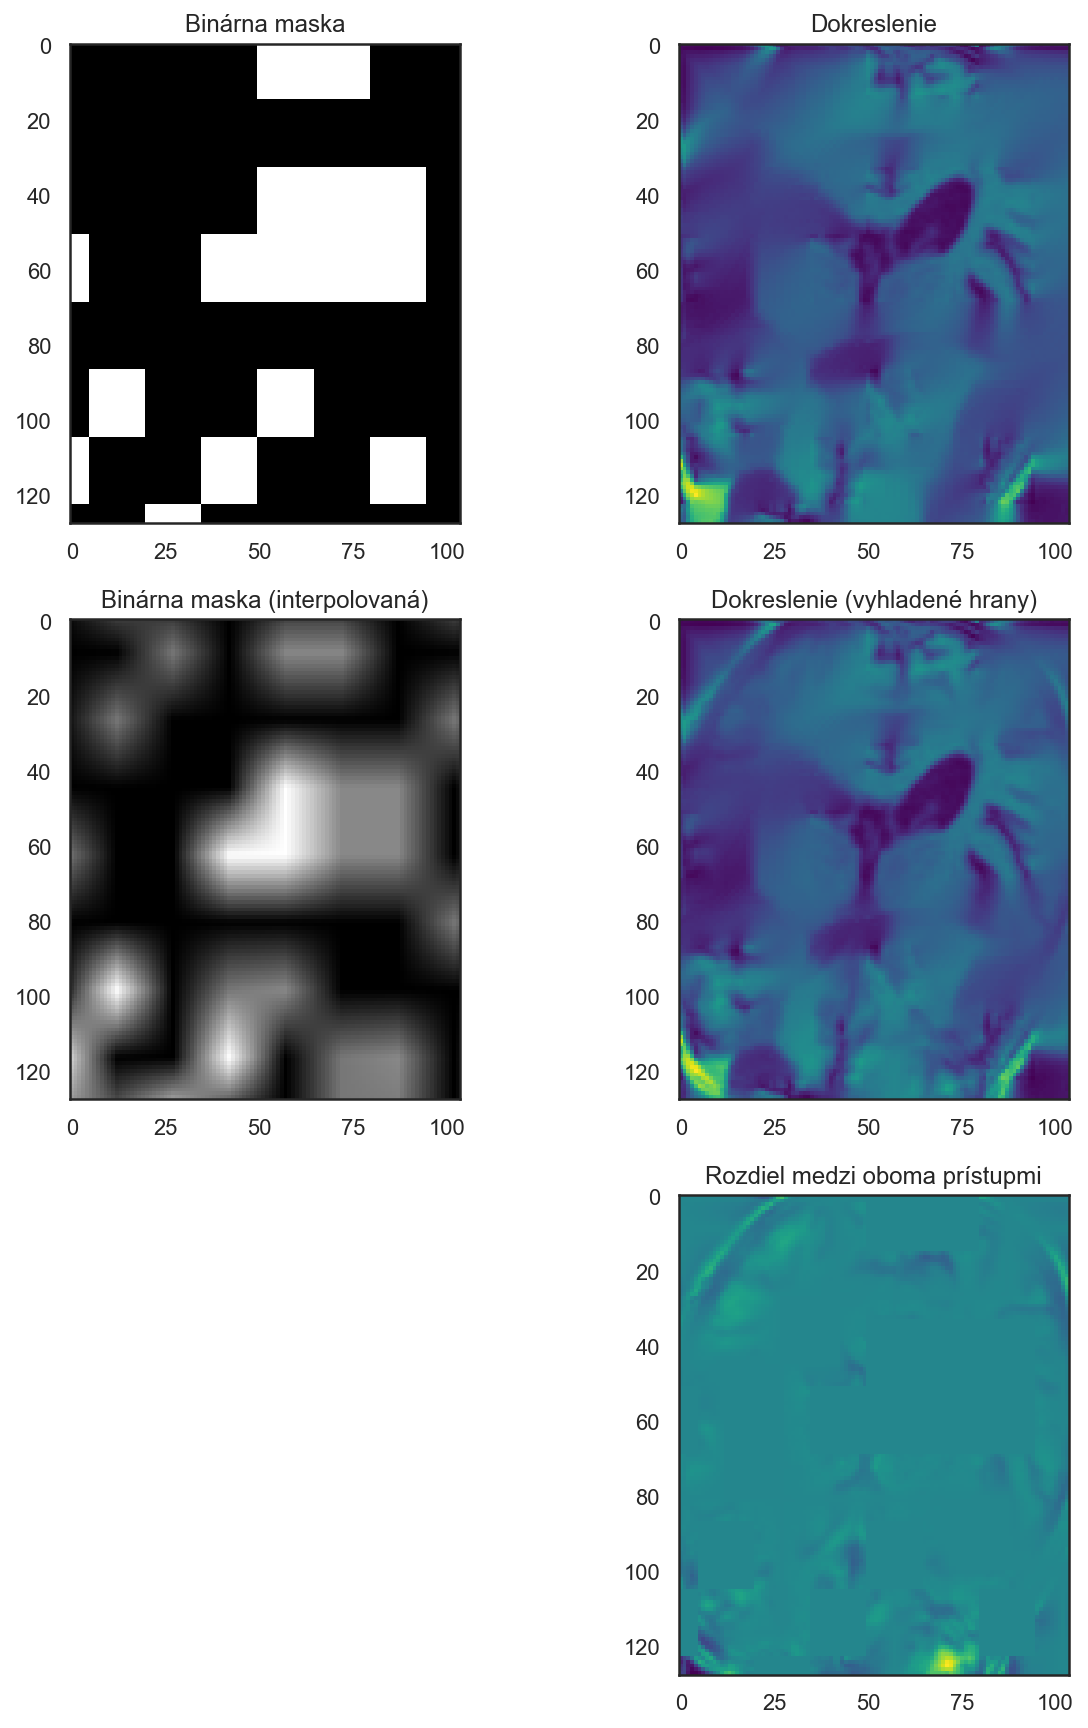
\includegraphics[width=13cm]{assets/images/inpaint_soft_corners.png}
    \caption{Príklad vyhladzovania hrán dokreslenia, alebo splynutie dokreslenia s pôvodným snímkom (štvrtý snímok)). Druhý snímok sobrazuje ostré hrany po dokreslení - bez splývania s obrázkom.}
    \label{fig:inpaint_soft_corners}
\end{figure}

\begin{figure}[h!]
    \centering
    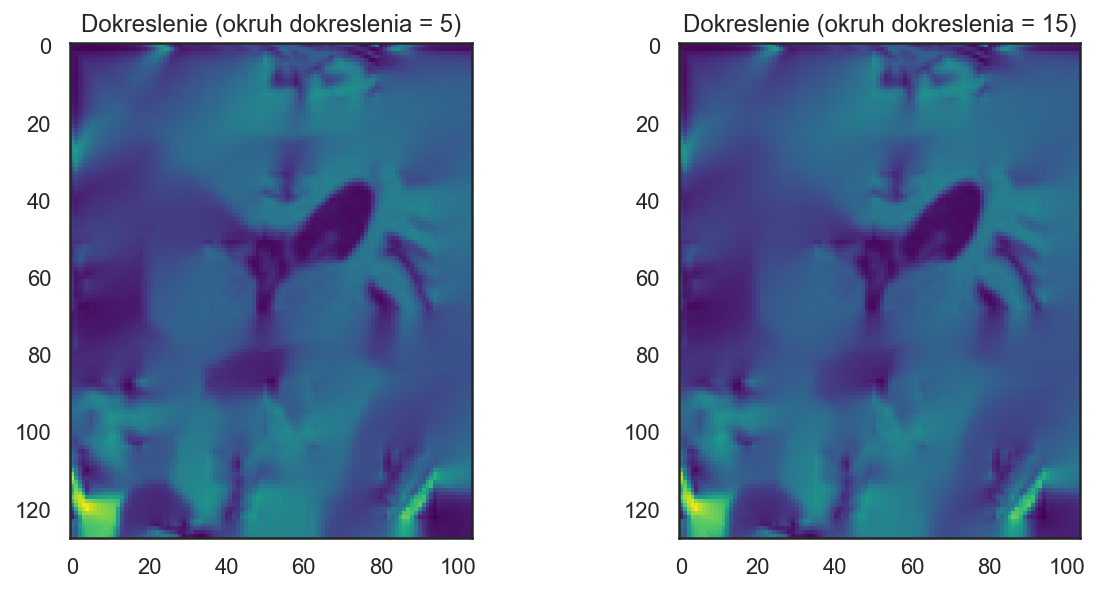
\includegraphics[width=13cm]{assets/images/inpaint_radius.png}
    \caption{Porovnanie okruhov dokreslenia (parameter \textit{inpaint\_radius}), rozdiel vo výsledku nie je veľmi viditelný, avšak s väčśím oruhom dokreslenia je generovanie rádovo pomalšie. (pri generovaní bolo vypnuté splynutie dokreslenia so snímkom aby bol rozdiel aspoň trochu viditeľný)}
    \label{fig:inpaint_radius}
\end{figure}

\begin{figure}[h!]
    \centering
    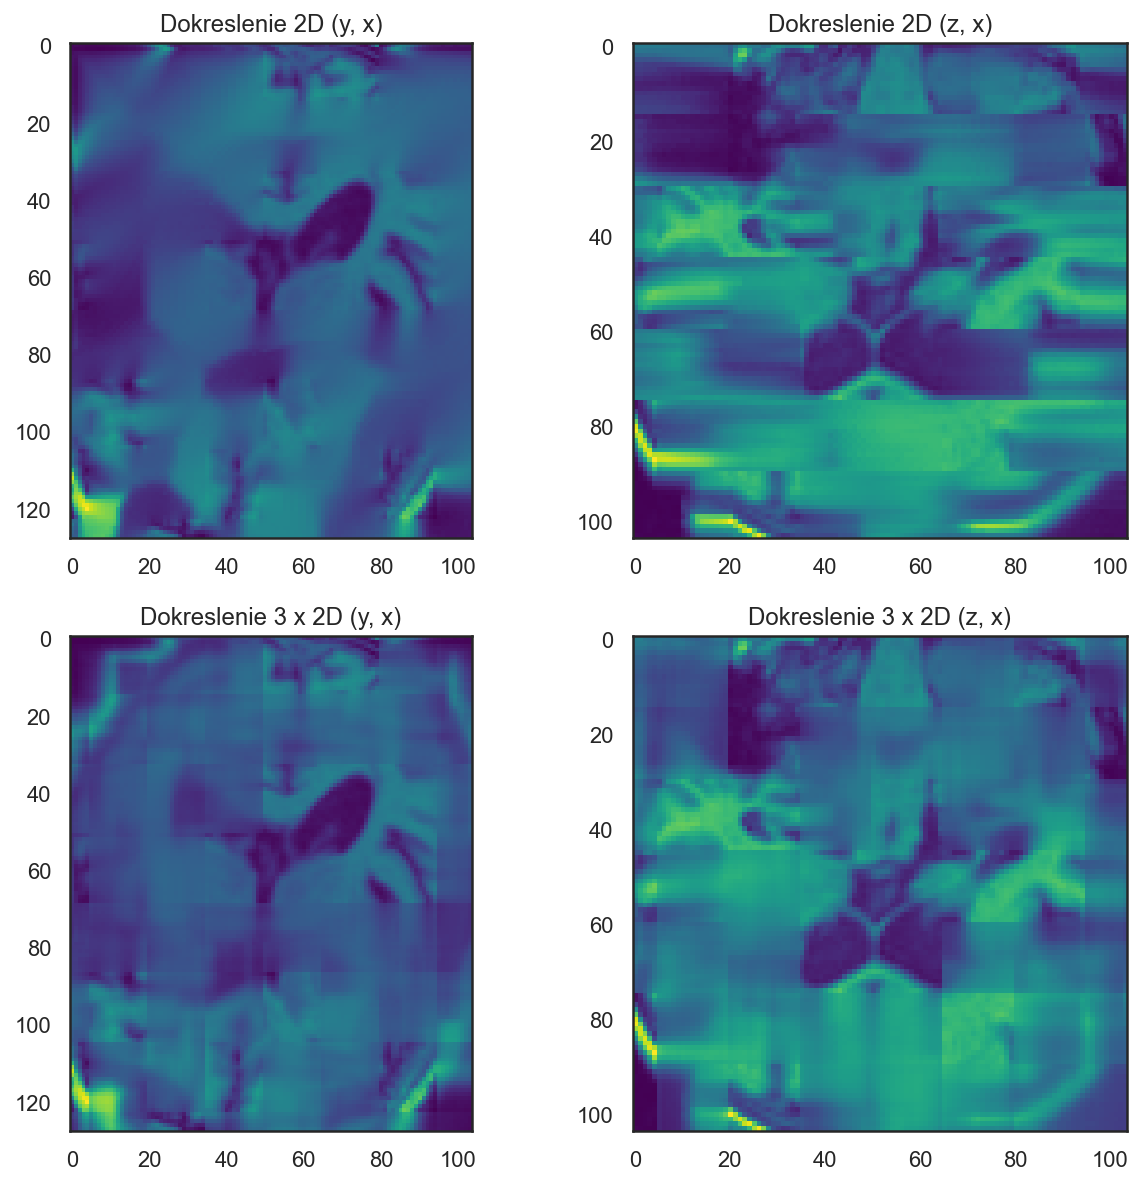
\includegraphics[width=13cm]{assets/images/inpaint_3x_2d.png}
    \caption{Porovnanie 2D dokreslenia (iba v jednej dimenzii) a spriemerovaného 3x 2D dokreslenia (v každej dimenzii). Použitie iba 2D dokreslenia je kvalitné iba v jednej dimenzii a v ostatných je deštruktívne - vytvára ostré hrany. Použitie 3x 2D dokreslenia a spriemerovanie pre každý voxel produkuje celkom dobré dokreslenia po všetkých dimenziách.}
    \label{fig:inpaint_3x_2d}
\end{figure}

\paragraph{Prekrytie dokreslenej masky a čiernej masky s obrázkom}

\subsection{Vytvorenie tepelných máp}

% TODO:

\section{Model na detekciu Alzheimerovej choroby na základe MRI snímkov}